%%%%%%%%%%%%%%%%  DISCUSSION  %%%%%%%%%%%%%%%%%%%%%
\chapter{Discussion} \thispagestyle{chapterpage}
\label{chapter:discussion}

\section{Convergence tests}
\label{section:discussion_convergence_tests}
We restate the viscosity residual from Equation (\ref{eq:residual_two_phase_transport}) with simplified notation:
\begin{equation} \label{eq:residual_two_phase_transport_simple}
R(S^{n+1};q_i,q_o,M,\tau) = S^{n+1} - S^{n} + \tau \left(q_o f_w(S^{n+1}) + q_i\right) = 0
\end{equation}
Here $\tau$ is defined by
\begin{equation*}
\tau = \frac{\Delta t}{m(V) \phi_V}.
\end{equation*}
The dynamics of the fluid flow is embedded in the last term of the Equation (\ref{eq:residual_two_phase_transport_simple}), i.e. $\tau \left(q_o f_w(S^{n+1}) + q_i\right)$. We call this the \emph{flow term} of the transport equation. The observations from the convergence tests in Section \ref{section:numerical_results_convergence_tests} indicates that the cell saturation from the previous transport step can be a determining factor for the root placement. We now seek to investigate under which circumstances this is the case. Since the saturation $S^n \in [0,1]$, we have a well defined range for the size of the two first terms in Equation (\ref{eq:residual_two_phase_transport_simple}). This implies that the old cell saturation $S^n$ is significant when $\tau \left(q_o f_w(S^{n+1}) + q_i\right) \approx 1$, in the sense that the size of the flow term is of the same order of magnitude as the number $1$. Of course, $S^{n+1} = S^n$ when $\tau \left(q_o f_w(S^{n+1}) + q_i\right) = 0$. Likewise, when the flow term is much larger than $1$, the solution $S^{n+1}$ is completely dominated by the fractional flow function $f_w$ and the flux terms $q_i$ and $q_o$. These facts explains the observations made based on the convergence plots in Section \ref{section:numerical_results_convergence_tests}. As stated, the size of the flow term in Equation (\ref{eq:residual_two_phase_transport_simple}) is determined by the incoming and outgoing fluxes, and the factor $\tau$. The fluxes measure the magnitude of flow in and out of the current cell, while $\tau$ gives the time-volume scale of the flow. That is, $\tau$ measures the number of seconds the fluxes $q_i$ and $q_o$ are allowed to move across the cell boundaries per volume unit of the cell. In practice this leads to small cells being drained faster than larger cells, and a larger flow in each iteration for large time steps.

It is of interest to know \emph{a priori} under which circumstances the old saturation value is a good starting guess for the root finders. The idea is that different combinations of the flux and time scale magnitudes causes the flux term in the transport equation to have varying significance.

We start by treating the case $q_i = 0$. Now, Equation (\ref{eq:residual_two_phase_transport_simple}) becomes
\begin{equation*}
R(S^{n+1}) = S^{n+1} - S^{n} + \tau q_o f_w(S^{n+1}) = 0
\end{equation*}
If $\tau q_o \gg 1$ the equation reduces to $f_w(S^{n+1}) = 0$, which will be positive and much larger than unity for all but the smallest $S^{n+1}$. As $S^{n+1}$ goes to zero, the influence of $S^{n+1}$ becomes more significant, pulling the slightly to the right. The root remains close to zero in this case. With $\tau q_o$ of the same order of magnitude as $S^n$ the root will be close to $S^n$. 

Now, if $q_o = 0$ the residual in Equation (\ref{eq:residual_two_phase_transport_simple}) reduces to
\begin{equation*}
R(S^{n+1}) = S^{n+1} - S^{n} + \tau q_i = 0 ~ \Rightarrow S^{n+1} = S^n - \tau q_i 
\end{equation*}
By definition $q_i \leq 0$, so this requires $0 \leq - \tau q_i  \leq 1 - S^n$. The lower bound is always satisfied since $\tau \geq 0$.

Having treated the zero flux cases we now assume $q_o,q_i \neq 0$. Dividing the residual in Equation (\ref{eq:residual_two_phase_transport_simple}) by $q_i \gg 1$ we get
\begin{equation*}
\frac{S^{n+1}}{q_i} - \frac{S^n}{q_i} + \tau \frac{q_o}{q_i} f_w(S^{n+1}) + \tau = 0.
\end{equation*}
Since saturations are in the range $[0,1]$ the two first terms become very small. In addition the scaled time step $\tau$ is usually orders of magnitude larger than unity, implying that the first two terms can be removed. \textbf{What about the case when $f_w$ is small over a larger range, i.e. with $M > 1$? For the right combination of fluxes the outward flux term might become small even with $\tau \gg 1$.} \todoinline{Give some kind of substance for the $\tau$ claim.} The resulting equation becomes
\begin{equation} \label{eq:flux_dominated_residual}
\frac{q_o}{q_i} f_w(S^{n+1}) + 1 \approx 0,
\end{equation}
a second order equation in $S^{n+1}$ when assuming quadratic relative permeabilities $k_{rl}$. At this point an important fact is revealed, namely that the absolute value of the incoming flux $q_i$ must be close to $q_o$. That is, the ratio $r_q$ defined by
\begin{equation*}
r_q \coloneqq \frac{q_o}{q_i},
\end{equation*}
must be close to or much greater than unity since $\lvert r_q \rvert \ll 1$ in Equation (\ref{eq:flux_dominated_residual}) would lead to the contradiction $1 \approx 0$. With $\lvert r_q \rvert \gg 1$ the fractional flow term dominates, bringing the solution $S^{n+1}$ close to zero. Finally we arrive at the case where $\lvert r_q \rvert \approx 1$. Now the flux dominated residual in Equation (\ref{eq:flux_dominated_residual}) is a second order equation in $S^{n+1}$,
\begin{equation*}
r_q S^2 +  S^2 + M(1-S)^2 = (1+M+r_q)S^2 - 2MS + M = 0
\end{equation*}
which can be solve using the well known quadratic equation, giving:
\begin{equation*}
S_{\pm} = \frac{2M \pm \sqrt{4M^2 - 4 M (1+M+r_q)}}{2(1+M+r_q)} = \frac{M \pm \sqrt{ - M (1+r_q)}}{1+M+r_q}
\end{equation*}
The special case $1+M+r_q = 0$ implies $S = 1/2$. In the following we therefore assume $1+M+r_q \neq 0$. In order for the quadratic formula to yield a solution we need $r_q \leq -1$. We define a number $\alpha = \lvert r_q \rvert / M$, such that
\begin{equation*}
S_{\pm} = \frac{1 \pm \sqrt{\alpha}}{1 - \alpha},
\end{equation*}
and $\alpha \geq 0$. The degenerate case $\alpha = 0$ gives $S_{\pm} = 1$. Otherwise, with $\alpha > 0$ we see that
\begin{equation*}
S_{+} = \frac{1 + \sqrt{\alpha}}{1 - \alpha}.
\end{equation*}
The saturation $S_+$ is clearly greater than unity for $0  < \alpha < 1$, further $\alpha = 1$ corresponds to $M + 1 + r_q = 0$, so $S_+ = 1/2$ as stated above. Last, with $\alpha > 1$ we get a positive numerator and a negative denominator, yielding a negative $S_+$, and invalid saturation solutions. We thus only consider the solution
\begin{equation*}
S = S_{-} = \frac{1 - \sqrt{\alpha}}{1 - \alpha}.
\end{equation*}
The case $\alpha = 1$ still gives $S = 1/2$. With $0 < \alpha \neq 1$ we get $0 < S < 1$ since $1 - \sqrt{\alpha} < 1 - \alpha$, which holds because $\sqrt{x} < x$ for $x > 1$ and $\sqrt{x} > x$ for $0 < x < 1$. This lengthy discussion has provided a simple formula for an approximate solution to the transport equation, the point being that it can be used as to generate a better initial guess than the old cell saturation $S^n$ provides. It is important to note that the criteria for the validity of the improved initial guess are rather restrictive, so the implementation should be given special attention.

%%%%%%%%%%%%%%%%%%%%%%%%%%%%%%%%%
\noindent\makebox[\linewidth]{\rule{\textwidth}{0.4pt}}

\begin{itemize}
\item $q_i = 0$: $S^n$ dominates on the left hand side. If $\tau q_o$ is small the solution is dominated by init guess. Otherwise the solution is close to zero.
\item $q_o = 0$: $q_i$ must be $\approx 1$ for a solution to exist. $S^n$ is important, at least.
\item $\vert q_i \vert \gg 1$: $q_o$ must balance, solve quadratic equation.
\item $\vert q_o \vert \gg 1$: The transport flux term dominates. Need $q_i \approx q_o$ or much lower. Solve quadratic.
\end{itemize}

It is of interest to know \emph{a priori} under which circumstances the old saturation value is a good starting guess for the root finders. We investigate this by assuming $q_o, q_i \gg 1$. Then, dividing Equation (\ref{eq:residual_two_phase_transport_simple}) by $q_o$ we obtain
\begin{equation*}
\frac{S^{n+1}}{q_o} - \frac{S^n}{q_o} + \tau f_w(S^{n+1}) + \tau \frac{q_i}{q_o} = 0.
\end{equation*}
Since $q_0 \gg 1$, $\frac{S^{n+1}}{q_o} \ll 0$ and $\frac{S^n}{q_o} \ll 1$. Having assumed quadratic relative permeabilities $k_{rl}$ the shape of the fractional flow function $f_w(S;M)$ is as shown in Figure \ref{fig:fractional_flow_wrt_viscosity_ratio} for varying viscosity ratios $M$. 
%\begin{figure}[ht]
\tikzsetnextfilename{fractional_flow_wrt_viscosity_ratio}
\centering
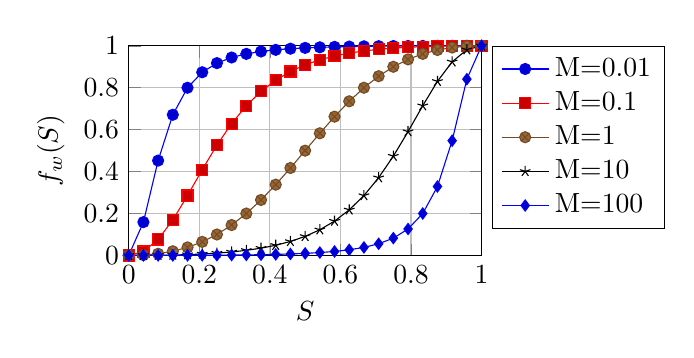
\begin{tikzpicture}
\begin{axis}[
	width=0.5\textwidth,
	height=0.35\textwidth,
	xlabel={$S$},
	ylabel={$f_w(S)$},
	xmin = 0,
	xmax = 1,
	ymin = 0,
	ymax = 1,
	domain = 0:1,
	%samples = 100,
	grid = major,
	legend style={
		cells={anchor=west},
		legend pos=outer north east,
	}
	]
	\addplot {x^2/(x^2+0.01*(1-x)^2)};
	\addplot {x^2/(x^2+0.1*(1-x)^2)};
	\addplot {x^2/(x^2+1*(1-x)^2)};
	\addplot {x^2/(x^2+10*(1-x)^2)};
	\addplot {x^2/(x^2+100*(1-x)^2)};
	\legend{M=0.01,M=0.1,M=1,M=10,M=100}
\end{axis}
\end{tikzpicture}
\caption{The fractional water flow function $f_w$, Equation (\ref{eq:fractional_flow_function}), with quadratic $k_{rl}$ and viscosity ratio $M$, Equation (\ref{eq:viscosity_ratio}).}%
\label{fig:fractional_flow_wrt_viscosity_ratio}%
\end{figure}%
We observe that $M > 1$  gives $f_w$-values closer to unity on the left hand side, while $M < 1$ brings the left hand side values of $f_w$ close to zero, leaving a smaller region close to unity for $S > \frac{1}{2}$. Still, $f_w(S = 0;M) = 0$ for all $M > 0$.
The ratio of the fluxes is of special interest, so we define a ratio $r_q$ by
\begin{equation*}
r_q \coloneqq \frac{q_i}{q_o}.
\end{equation*} 
Now, if 
\begin{equation*}
 \tau \lvert r_q \rvert \approx  1,
\end{equation*} 
and since $\tau f_w \ll 1$ for ``small enough'' $S^{n+1}$, the old cell saturation $S^n$ is significant for determining the root. On the other hand, if 
\begin{equation} \label{eq:flux_term_dominance_criterium}
 \tau \lvert r_q \rvert \gg 1,
\end{equation}
we expect the root to be invariant under $S^n$ since this term will dominate the $S^n$ influence even for small $\tau f_w$. Thus the residual in Equation (\ref{eq:residual_two_phase_transport_simple}) is reduced to
\begin{equation*}
R(S^{n+1};q_i,q_o,M,\tau) \approx \tau \left(q_o f_w(S^{n+1}) + q_i\right) \approx 0
\end{equation*}
Dividing by $\tau$ and inserting the expanded form of the fractional flow function from Equation (\ref{eq:fractional_flow_function_expanded}) we arrive at an equation for the saturation $S^{n+1}$:
\begin{equation*}
 q_o \frac{\lambda_w(S^{n+1})}{\lambda_w(S^{n+1}) + \lambda_o(S^{n+1})} + q_i \approx 0.
\end{equation*}
Multiplying by the total mobility and inserting the mobility definition from Equation (\ref{eq:mobility}) we obtain a second order equation for the updated water saturation, here abbreviated $S$ for notational ease:
\begin{equation*}
 q_o S^2 + q_i \left[ S^2 + M (1-S^{n+1})^2 \right]  =  (q_o + q_i + M q_i) S^2 - 2 M q_i S + Mq_i  \approx 0.
\end{equation*}
If the incoming flux is zero, the equation is rendered invalid, since the criterium in Equation (\ref{eq:flux_term_dominance_criterium}) must hold. This allows us to divide the second order equation by $q_i$, such that
\begin{equation*}
\left(\frac{1}{r_q} + M + 1\right) S^2 - 2 M S + M  \approx 0.
\end{equation*}
Using the well known quadratic formula we obtain
\begin{equation*}
S_{\pm} = \frac{ 2M \pm \sqrt{4M^2 - 4 M (M+1+1/r_q)} }{2 (M + 1 + 1/r_q)} = \frac{ M \pm \sqrt{-M(1 + 1/r_q) } }{ M + 1 + 1/r_q } 
\end{equation*}
Since $M > 0$ we need 
\begin{equation*}
1 + \frac{1}{r_q} \leq 0 ~ \Rightarrow r_q \geq -1.
\end{equation*}
By definition the incoming flux in the residual formulation is negative, $q_i \leq 0$, and the outgoing flux is positive, $q_o \geq 0$. Thus, we get a lower and upper bound for the flux ratio $r_q$:
\begin{equation} \label{eq:flux_ratio_bound}
-1 \leq r_q \leq 0.
\end{equation}
Now, 
